\begin{figure}[t]
 \centering
 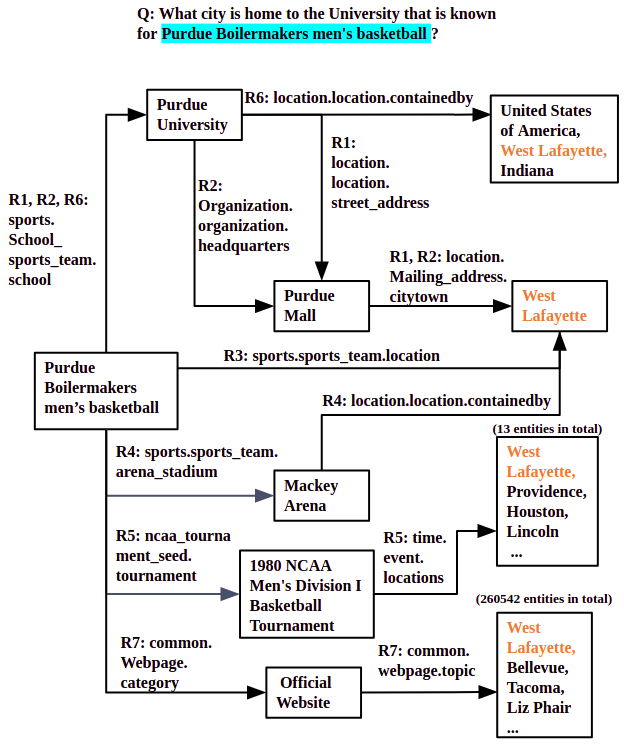
\includegraphics[width=1\linewidth]{figs/fig1.png}
 \caption{One QA example with Multiple Relation Paths from \textsc{ComplexWebQuestion}-1.1. The blue color highlighted is the extracted topic entity. Each square represents an entity, and the arrows represent the relations. Relation path $\mathbf{p}^1$ to $\mathbf{p}^4$ are the correct ones containing meaningful relation paths to the final answer. $\mathbf{p}^5$ and $\mathbf{p}^6$ are the ``second choice'' paths that generate a larger final answer set containing some wrong entities. $\mathbf{p}^7$ is the wrong one as its relation path is totally not interpretable and the answer set is huge.}
 \label{QAPaths}
\end{figure}

\section{Introduction}

Knowledge-based question answering (KBQA) is the task of finding answers to questions by processing a structured knowledge base $\mathcal{KB}$. %where the beliefs are stored as triples containing two entities and the relation linking them. 
A $\mathcal{KB}$ consists of a set of entities $\mathcal{E}$, a set of relations $\mathcal{R}$, and a set of literals $\mathcal{S}$. A knowledge base fact is defined as $(h,r,t)$, where $h\in \mathcal{E}$ is the head entity, $t \in \mathcal{E} \bigcup \mathcal{S}$ is the tail entity/literal, and $r\in \mathcal{R}$ is the directed relation between $h$ and $t$. To answer a simple single-relation question (\emph{i.e.} a 1-hop question) such as: \textit{``Who is the president of the United States?''}, %a KBQA system first identifies the topic/focus entity (\emph{i.e.} United States) and the relation (\emph{i.e.} ``president '') asked in the question, then searches for the entity by matching the entity-relation tuple $\textless$United States, president, $?\textgreater$ over KB. \kalpa{use of a topic entity is approach specific. Many KBQA systems exist that do not use topic entity. E.g., template based QA}
a typical KBQA system first identifies the entity (\emph{i.e.} United States) and the relation (\emph{i.e.} ``president'') asked in the question, and then searches for the answer entity by matching the entity-relation tuple $\textless$United States, president, $?\textgreater$ over $\mathcal{KB}$.


While a single-hop question can be answered by searching a predicate relation in $\mathcal{KB}$, it is much harder to answer more complex multi-hop questions containing multiple entities and relations with constraints. For instance, for complex compositional questions, it is not easy to extract all the relations correctly together with their head and tail entities in the right order. For complex conjunction questions that requires a conjunction of multiple evidences, it is even more difficult to correctly extract all the reasoning paths included.

Most prior work on multi-hop KBQA focuses on learning a single given ground truth relation path for each question, and outputting the most possible reasoning path during prediction \cite{DBLP:conf/coling/ZhouHZ18,DBLP:journals/corr/abs-1801-09893,DBLP:conf/adbis/YuHYZW18,DBLP:conf/ijcai/LanW019}. However, it is common that $\mathcal{KB}$ has many alternative paths leading to the correct answer, of various reasoning quality. These alternative reasoning paths are usually not provided as ground truth by the human annotators. %It is hard to pre-define the maximum number of hops in a complex question because different questions may need different number of hops to reach their answers.
%\kechen{list a few problems (1) it hard to control number of hops. (2) how to decompose a complex question into sub-question. (3) ...} 
%\kechen{add something to explain why the above two points lead to decomposing into two sub-tasks?}
 %with random walks \cite{DBLP:conf/emnlp/GardnerTKM13} or is formulated as a Markov decision process (MDP) based reinforcement learning problem~\cite{DBLP:conf/emnlp/XiongHW17}.
%\kechen{Most of the existing KBQA systems cannot handle these two issues simultaneously. People have to pre-define different rules to solve different type of complex querys. For example, list a few work using different pre-defined strategy to solve complex QA.}%1. use different model to train, 2. neural program
%traditional approaches consider all the paths and search for the best path among them, where their searching algorithms either leverage path-ranking algorithms with random walks \cite{DBLP:conf/emnlp/GardnerTKM13} or is formulated as a Markov decision process (MDP) based reinforcement learning problem~\cite{DBLP:conf/emnlp/XiongHW17}. Since the complexity of the searching process can grow exponentially when the number of hops increase, some recent researches add decision markers or a terminal relation to decide whether a searching path should terminate or continue, in order to reduce the searching space and complexity \cite{DBLP:conf/naacl/ChenCCNK19}.
%It is commonly observed that, by using the above mentioned algorithms, the extracted relation path may not always be the best one or even can be a wrong one. The main reason is because during training, for one question, their models are trying to learn and fit to only one possible relation path, which is given as its ground truth. \kechen{while during prediction only predict one path}In reality, however, it is always possible that there exists many other relation paths leading to the answer, which are not given as ground truth. 
For example, figure \ref{QAPaths} shows 7 relation paths $\mathbf{p}^n={e^n_0\rightarrow r^n_1 \rightarrow e^n_1 \rightarrow \cdots \rightarrow e^n_{ans}}\ (n=\lbrace 1, \dots, 7 \rbrace)$ leading to an answer set containing the correct answer \textit{``West Lafayette''} for a given question \textit{``What city is home to the University that is known for Purdue Boilermakers men's basketball?''}%\footnote{An exchangeable way to define relation path is omitting entities in the definition, because entity is determined by given the topic entity, relations, and the knowledge base. For simplicity, we simplify this relation path definition as a list of sequential relations $(r_{1}^n, r_{2}^n, \cdots, r_{T}^n)$ in the following part of this paper.}
, but only the relation path $\mathbf{p}^1$ is labeled as the correct path in the dataset. A model trained with only $\mathbf{p}^1$ as supervision is likely to miss paths which are also valid. For example, it will probably map map a similar question \textit{``What city is home to the stadium that is known for Los Angeles Lakers?''} to path $\mathbf{p}^1$, but fail to associate it with $\mathbf{p}^3$ or $\mathbf{p}^4$, because $\mathbf{p}^3$ or $\mathbf{p}^4$ contain different types of relations. Apparently, $\mathbf{p}^1$ is a wrong reasoning path for the that test question.

As the example shown in Figure \ref{QAPaths}, there are four paths ($\mathbf{p}^1$,$\mathbf{p}^2$,$\mathbf{p}^3$,$\mathbf{p}^4$) pointing to the exact answer set containing only the answer entity, and thus can be treated as ground truth paths when training. Comparatively, relation paths $\mathbf{p}^5$ and $\mathbf{p}^6$ lead to a larger final entity set containing the correct answer \textit{``West Lafayette''} but also other entities. These two paths can be considered as inferior to the top 4 paths; however, it is still worth including them in the training as a ``second choice'', as it is not difficult to extract the correct answer from final sets by additional post-processing. For example, a simple filter can be applied to filter out \textit{``United States of America''} and \textit{``Indiana''} from the predicted set, as they are not cities. Path $\mathbf{p}^7$ is a bad because it is totally not interpretable, in addition to the final answer set being exaggeratedly large with invalid answers. Hence, Path $\mathbf{p}^7$ should not be considered as a training path for this question. Unfortunately, it is not possible for any existing models to use multiple good/inferior paths, but not the bad ones, since current models are only trained with a single path for each question answer pair.

%Although someone may claim that we can use multiple relation paths as ground truths for one question to improve the coverage and performance, it is still not feasible to label all valid relation paths considering the complexity of ground truth label preparation. 
%\kechen{combine this paragraph with the next paragraph? now we have two separate paragraphs to first introduce the issue and then use an example to explain it. should we combine them together?}

In this paper, we propose an end-to-end multi-hop KBQA system, which can leverage the training information from multiple relation paths and luckily without using relation path annotation. We model the relation path as a latent variable, and propose supporting training and prediction methods. The system can output diverse relation paths, and reward the ``better'' paths over the inferior ones by assigning ``better'' paths higher probabilities. Our method can be applied to most KBQA systems to predict the answer, and can be used with any model architecture. We achieve strong performance on three popular KBQA datasets. Experimental results show that our model performs especially well on multi-hop question, and in particular on complex questions that cannot be solved with a single reasoning path.

Our method doesnt need training paths annotation (only the question, and head and final entities), since it can sample the paths from the $\mathcal{KB}$ graph. This is of enormous pratical importance, because in practice questions and answers are easy to collect (sometimes for free), but path annotation is very labor-intensive and expensive. 

%\kechen{Especially, we show that our model perform extremely well on difficult dataset vs. simple dataset, multi-hop question vs. single question, and multiple path question vs. single path question.} %taking the size of their answer set into consideration, \emph{i.e.} the larger is the final answer set, the worse is a relation path, as it contains more irrelevant answer information. \kechen{modify the last sentence} %We also use a sampling approach to filter the wrong paths like $R_8$ in our example. 
% Specifically, we make the following contributions:\\
% 1. We introduce a novel multi-hop KBQA structure, which can predict the relation sequence of any length without pre-defining the number of maximum hops and generate final answers at the last hop.\\
% 2. We design a novel loss function using latent variables, such that the system can be trained without being given any ground truth relation path, or by leveraging more valid training paths information even if one ground truth path is given. We also give detailed analysis to demonstrate the benefits of using the new loss function.\\
% 3. We achieve state-of-the-art performance on three popular KBQA dataset containing single-hop and multi-hop questions.
%Specifically, we make the following contributions:
%\begin{enumerate}
%  \item We introduce a novel multi-hop KBQA system, which can leverage the information from multiple relation paths. %predict the relation sequence of any length without pre-defining the number of maximum hops and generate final answers at the last hop.
%  \item We design a novel loss function and the corresponding training and prediction methods. Detailed analysis is given to demonstrate the benefits of using this new loss function.
%  \item We achieve state-of-the-art performance on three popular KBQA datasets for single-hop and multi-hop questions.
%\end{enumerate}
